%%%%%%%%%%%%%%%%%%%%%%%%%%%%%%%%%%%%%%%%%%%%%%%%%%%%%%%%%%%%%%%%%%%%%%
% hydro_comp_numerics_mwr.tex --  LaTeX-based template for submissions to American 
% Meteorological Society journals
%
% Template developed by Amy Hendrickson, 2013, TeXnology Inc., 
% amyh@texnology.com, http://www.texnology.com
% following earlier work by Brian Papa, American Meteorological Society
%
% Email questions to latex@ametsoc.org.
%
%%%%%%%%%%%%%%%%%%%%%%%%%%%%%%%%%%%%%%%%%%%%%%%%%%%%%%%%%%%%%%%%%%%%%
% PREAMBLE
%%%%%%%%%%%%%%%%%%%%%%%%%%%%%%%%%%%%%%%%%%%%%%%%%%%%%%%%%%%%%%%%%%%%%

%% Start with one of the following:
% DOUBLE-SPACED VERSION FOR SUBMISSION TO THE AMS
\documentclass{ametsoc}

% TWO-COLUMN JOURNAL PAGE LAYOUT---FOR AUTHOR USE ONLY
%\documentclass[twocol]{ametsoc}

%%%%%%%%%%%%%%%%%%%%%%%%%%%%%%%%
%%% To be entered only if twocol option is used

\journal{mwr}

%  Please choose a journal abbreviation to use above from the following list:
% 
%   jamc     (Journal of Applied Meteorology and Climatology)
%   jtech     (Journal of Atmospheric and Oceanic Technology)
%   jhm      (Journal of Hydrometeorology)
%   jpo     (Journal of Physical Oceanography)
%   jas      (Journal of Atmospheric Sciences)	
%   jcli      (Journal of Climate)
%   mwr      (Monthly Weather Review)
%   wcas      (Weather, Climate, and Society)
%   waf       (Weather and Forecasting)
%   bams (Bulletin of the American Meteorological Society)
%   ei    (Earth Interactions)

%%%%%%%%%%%%%%%%%%%%%%%%%%%%%%%%
%Citations should be of the form ``author year''  not ``author, year''
\bibpunct{(}{)}{;}{a}{}{,}

%%%%%%%%%%%%%%%%%%%%%%%%%%%%%%%%

\usepackage{booktabs}
\usepackage{array}
\usepackage{siunitx}
\usepackage{float}


\usepackage{amsmath}
\usepackage{amssymb}
\usepackage{amsthm}

%\usepackage[squaren]{SIunits}
\usepackage{graphicx}
\usepackage{IEEEtrantools}
\usepackage{mdframed} % or, "mdframed"

%----------------------------------------------------------------------------
%---- Farben und Macros zur Textmarkierung ----------------------------------
%----------------------------------------------------------------------------
\usepackage{color}
\definecolor{light}{gray}{0.50}
\definecolor{heavy}{gray}{0.35}
\definecolor{black}{gray}{0.0}
\definecolor{dgreen}{rgb}{0.0,0.7,0}
\definecolor{dred}{rgb}{0.9959,0,0}
\definecolor{green}{rgb}{0.0,0.99599,0.0}
\definecolor{purple}{rgb}{0.6,0.0,0.4}

\newcommand{\red}[1]{\textcolor{dred}{#1}}
\newcommand{\green}[1]{\textcolor{green}{#1}}
\newcommand{\dgreen}[1]{\textcolor{dgreen}{#1}}
\newcommand{\purple}[1]{\textcolor{purple}{#1}}
\newcommand{\blue}[1]{\textcolor{blue}{#1}}
\newcommand{\black}[1]{\textcolor{black}{#1}}
\newcommand{\grey}[1]{\textcolor{heavy}{#1}}
\newcommand{\lightgrey}[1]{\textcolor{light}{#1}}

\theoremstyle{definition}
\newtheorem{algorithm}{Algorithm}


%----------------------------------------------------------------------------
%---- Kommentare ------------------------------------------------------------
%----------------------------------------------------------------------------

\newcommand{\klein}[1]{\textcolor{blue}{#1}}
\newcounter{kleincommentno}
\setcounter{kleincommentno}{1}
\newcommand{\kleincomment}[1]{{\small\bfseries\textcolor{blue}{ {\small\bfseries${}^{[\arabic{kleincommentno}]}$}}%
\marginpar{\textcolor{blue}{{\small{\bfseries[\arabic{kleincommentno}]}\ \small #1}}\addtocounter{kleincommentno}{1}}}}

\newcommand{\benacchio}[1]{\textcolor{red}{#1}}
\newcounter{benacchiocommentno}
\setcounter{benacchiocommentno}{1}
\newcommand{\benacchiocomment}[1]{{\small\bfseries\textcolor{red}{ {\small\bfseries${}^{[\arabic{benacchiocommentno}]}$}}%
\marginpar{\textcolor{red}{{\small{\bfseries[\arabic{benacchiocommentno}]}\ \small #1}}\addtocounter{benacchiocommentno}{1}}}}

%----------------------------------------------------------------------------
%---- Eigene Macros ---------------------------------------------------------
%----------------------------------------------------------------------------
\newcommand{\hsc}{h_{\rm sc}}
\newcommand{\order}[1]{^{(#1)}}
\let\dss=\displaystyle

\renewcommand{\vector}[1]{\relax\ifmmode\mathchoice
{\mbox{\boldmath$\displaystyle#1$}}
{\mbox{\boldmath$\displaystyle#1$}}
{\mbox{\boldmath$\scriptstyle#1$}}
{\mbox{\boldmath$\scriptscriptstyle#1$}}\else
\hbox{\boldmath$\textstyle#1$}\fi}

\newcommand{\eq}[1]{(\ref{#1})}

\newcommand{\vect}[1]{{\mathbf{#1}}}

\newcommand{\cbar}{\overline{c}}
\newcommand{\thetabar}{\overline{\theta}}
\newcommand{\thetatilde}{\widetilde{\theta}}

\newcommand{\vk}{\vect{k}}
\newcommand{\vu}{\vect{u}}
\newcommand{\vv}{\vect{v}}
\newcommand{\vx}{\vect{x}}

\newcommand{\vV}{\vect{V}}

\newcommand{\ubar}{\overline{u}}
\newcommand{\vbar}{\overline{v}}

\newcommand{\advection}[1]{\mathcal{A}\left[#1\right]}
\newcommand{\advectionNum}[1]{\widetilde{\mathcal{A}}\left[#1\right]}
\newcommand{\rhs}[1]{\mathcal{R}\left[#1\right]}
\newcommand{\source}[1]{S\left(#1\right)}
\newcommand{\Id}{{\rm Id}}

\newcommand{\pprime}{p'}
\newcommand{\halff}{\frac{1}{2}}
\newcommand{\half}{1/2}
\newcommand{\quart}{\frac{1}{4}}
\newcommand{\eightth}{\frac{1}{8}}

\newcommand{\ie}{\emph{i.e.}}

\newcommand{\Nsq}{N^2}
\newcommand{\Nscsq}{(\tau N)^2}

\newcommand{\chibar}{\overline{\chi}}
\newcommand{\chitilde}{{\widetilde \chi}}
\newcommand{\chiprime}{{\chi'}}
\newcommand{\Xtilde}{{\widetilde X}}
\newcommand{\Thetabar}{\overline{\Theta}}
\newcommand{\Thetatilde}{{\widetilde \Theta}}
\newcommand{\pibar}{\overline{\pi}}
\newcommand{\pitilde}{{\widetilde \pi}}
\newcommand{\pihat}{\widehat{\pi}}
\newcommand{\piprime}{\pi'}
\newcommand{\piprimehat}{\widehat{\pi}'}

\newcommand{\Uhat}{\widehat{U}}

\newcommand{\pp}[2]{\frac{\partial #1}{\partial #2}}
\newcommand{\ppn}[3]{\frac{\partial^{#1} #2}{\partial #3^{#1}}}

\newcommand{\bigoh}[1]{\mathcal{O}\left(#1\right)}
\newcommand{\littleoh}[1]{{\scriptstyle\mathcal{O}}\left(#1\right)}

\newcommand{\reals}{\mathbb{R}}

\newcommand{\eps}{\varepsilon}
\newcommand{\rbeta}{\red{\vector{\beta}}}
\newcommand{\balpha}{\blue{\vector{\alpha}}}

\newcommand{\Lopfirst}{{\cal L}^{\rm 1st}}

%\newcommand{\Sol}{\boldsymbol{\mathcal{U}}}
\newcommand{\Sol}{\mathcal{U}}

\newcommand{\rfr}[1]{#1_{\text{ref}}}

\newcommand{\nablatilde}{{\widetilde\nabla}}

\newcommand{\dx}{{\Delta x}}
\newcommand{\dy}{{\Delta y}}
\newcommand{\dz}{{\Delta z}}
\newcommand{\dt}{{\Delta t}}

\newenvironment{falgorithm}
  {\begin{mdframed}\begin{algorithm}}
  {\end{algorithm}\end{mdframed}}



%%% To be entered by author:

%% May use \\ to break lines in title:

\title{A semi-implicit numerical model for small-to-planetary scale atmospheric dynamics}

%%% Enter authors' names, as you see in this example:
%%% Use \correspondingauthor{} and \thanks{Current Affiliation:...}
%%% immediately following the appropriate author.
%%%
%%% Note that the \correspondingauthor{} command is NECESSARY.
%%% The \thanks{} commands are OPTIONAL.

\authors{Tommaso Benacchio\correspondingauthor{Tommaso  Benacchio, MOX - Modelling and Scientific Computing,
Dipartimento di Matematica, Politecnico di Milano, via Bonardi 9, 20133 Milano, Italy}}

\email{tommaso.benacchio@polimi.it}

\affiliation{MOX - Modelling and Scientific Computing,
Dipartimento di Matematica, Politecnico di Milano, via Bonardi 9, 20133 Milano, Italy}

\extraauthor{Rupert Klein}

\extraaffil{FB Mathematik \& Informatik, Freie Universit\"at Berlin, Germany}

%%%%%%%%%%%%%%%%%%%%%%%%%%%%%%%%%%%%%%%%%%%%%%%%%%%%%%%%%%%%%%%%%%%%%
% ABSTRACT
%
% Enter your Abstract here

\abstract{We introduce a \klein{second-order numerical scheme for atmospheric motions at small to planetary scales. The finite volume model is conservative for mass, momentum, an density weighted potential temperature, it} uses time steps constrained by the advection speed only, and \klein{it} discretises the rotating compressible equations by evolving full variables without writing the system in terms of perturbations around a reference state. The algorithm reframes previous work by the authors into a sequence of implicit midpoint, advection, and implicit trapezoidal steps that allows for a time integration unconstrained by the internal gravity wave speed. Compared with exisiting approaches, results on a range of benchmarks of nonhydrostatic and hydrostatic-scale dynamics are competitive. The suite includes a new planetary-scale inertia-gravity wave test that highlights the properties of the scheme and its large time step capabilities. The development is a necessary step towards an all-scale blended multimodel solver for atmospheric dynamics with seamless access to reduced soundproof and hydrostatic dynamics.} 

\begin{document}

%% Necessary!
\maketitle


%%%%%%%%%%%%%%%%%%%%%%%%%%%%%%%%%%%%%%%%%%%%%%%%%%%%%%%%%%%%%%%%%%%%%
% MAIN BODY OF PAPER
%%%%%%%%%%%%%%%%%%%%%%%%%%%%%%%%%%%%%%%%%%%%%%%%%%%%%%%%%%%%%%%%%%%%%
%
\section{Introduction}
\label{sec:Intro}

%TBD 
% \cite{SmolarkiewiczEtAl2016}
% 
% Literature review re two-time level, full variables, no off-centering, conservative (and of what), second-order, advection-explicit.
% 
% Second-order accurate schemes rare. This is an extension of \cite{BenacchioEtAl2014} to address a gap in their formulation, but how novel is it? 





% Key points of the paper: 
% \begin{itemize}
% \item Semi-implicit scheme, only advection explicit
% \item Full variables advanced in time \\
%       \klein{We obtain the best results by running a redundant nodal pressure evolution
%       as is done in EULAG and FVM. With the most recent results we seem to get away with
%       the implicit trapezoidal rule for the time integration in the implicit part without
%       offset, which Piotr tells me they cannot do for all THEIR tests. Of course, they are
%       running different tests than us, so it remains to be seen how far we get with what
%       we have. Whenever I switch on synchronizations, I see spurious perturbations and
%       instabilities creep up. \\ 
%       Another point is that currently I am extracting a mean pressure profile both from 
%       the nodal and the cell-centered pressures that enter the momentum balances (for
%       cells and interface momenta, respectively). We will need to test whether we can
%       work with full variables there and/or whether the scheme runs robustly if we DYNAMICALLY
%       calculate the background state.}
% \item Unconditional time step stability w.r.t.\ acoustics, internal waves, Rossby waves\\
%       \klein{We surely should aim to demonstrate this through examples. Can we construct
%       rigorous arguments?}
% \item Background states \& perturbation variables are only auxiliary \\
%       \klein{Again, this we should be able to demonstrate. See two items up.}
% \item Mix of implicit midpoint and implicit trapezoidal rules \\
%       \klein{I am not so sure the approach is new as it is very close to the 
%       usual MAC-Projection + second project approach used by many others in the
%       ``approximate projection'' world, but I do think that viewing what we do from 
%       this angle might allow for improved understanding of the scheme's properties.}
% \item Borrowing ideas from EULAG/FVM
% \item \benacchio{(Mass-, horizontal momentum-,...?) Conservative} \\
%       \klein{Interesting point. We conserve $\rho$ and $\rho\theta$ for sure, but already
%       for momentum I am compromising, as I seem to need the Exner variable to get 
%       reliable implicit gravity. Here we may want to go back to your/Warren's theses,
%       and later discussions of mine where we show that one can have discretely equivalent
%       Exner and full pressure formulations under the psinc model. If we can pull this off
%       for the compressible case, too, and I am optimistic, then we would have a very nice
%       point.}
% \item Second-order, symplectic in the implicit part, no off-centering, no diffusion
% %\item \benacchio{No off-centering}
% \item Further aim: Step towards extending compr/psinc blended model formulation 
%       from \citep{BenacchioEtAl2014, KleinEtAl2014} to cover hydrostasy, geostrophy, as well
%       \citep[see][]{KleinBenacchio2016}.
% 
% \item Test with rotation and multiscale, Baldauf and Brdar 2016.
% 
% \item Very large test simulating planetary scales in a Cartesian framework, showing competitive behaviour of our scheme
% 
% \end{itemize}
% 
% \benacchio{We should perhaps better clarify how this makes the scheme
% different from all the other models that work with perturbations only,
% e.g. ENDGame works with the old time-step profiles as reference. In our case
% the decompositions \eq{eq:PerturbationVariables} and \eq{eq:BackgroundHydrostatics} are only
% instrumental to constructing the elliptic problems in the correction steps.
% I shall go into the bells and whistles of other schemes to understand how
% they carry forward perturbations more than we do.} 
% 
%  \klein{\bfseries We use the full conservation form to update $\chi$ in the advection step. In contrast, 
% $\chi'$ is used only to prepare for the implicit gravity time integration and is
% overwritten after a time step. In your scan of the literature, please have a look
% at how others do this. I believe that only Hilary is doing it similarly to us in 
% her paper with Shahrokhi, and maybe in her later cell-centered code(s). But this, too,
% we need to double-check. }
% 
% 
% Novelty/competitiveness: Two-time level, full variables, no off-centering, conservative (and of what), second-order, advection-explicit.
% Possible aspects of novelty/discussion are a) Novel combination of functionality b) results quality c) implementation d) speed/scalability (presumably comparable to a DG code but without the high-order capabilities) e) flexibility towards encapsulating different equation sets/ outlook for blending, data assimilation.

A significant challenge in the dynamical description and forecast of weather and climate lies in the inherent multiscale nature of atmospheric flows. Driven by stratification and rotation, physical processes arise around a large-scale state of horizontal geostrophic, vertical hydrostatic balance. The compressible Euler equations are deemed the most comprehensive model to describe the \klein{principal fluid dynamical features of the system before parameterizations of unresolved processes are added. On the one hand, these equations allow for buoyancy-driven internal gravity and pressure-driven sound wave adjustments}.  On the other hand, meteorologically relevant features such as cyclones and anticyclones in the midlatitudes \klein{involve motions} much slower than \klein{the sound speed}, thus forcing numerical stiffness into discretizations of the compressible model in the low Mach number regime. As a result, most if not all numerical schemes used in operational weather forecasting employ varying degrees of implicitness that enable stable runs with long time step sizes unconstrained by sound speed (see \cite{BenacchioEtAl2014} and references therein for a list \kleincomment{Shouldn't we cite some other review here?}). \klein{Typically, s}emi-implicit approaches integrate \klein{advective} transport explicitly \klein{and} then build an elliptic problem for the pressure variable by combining of the equations of the discrete system. The solution of the problem yields updates that are then replaced into the other variables. 

Examples of operational dynamical cores using semi-implicit time-integrations strategies are the ECMWF\footnote{European Centre for Medium-Range Weather Forecasts}'s IFS (\cite{Hortal2002}, that discretizes the hydrostatic primitive equations, and the UK Met Office's ENDGame \citep{WoodEtAl2013, BenacchioWood2016}. In particular, ENDGame  uses a double-loop structure in the implicit solver entailing four solves per time step in its operational incarnation, a strategy carried over in recent developments \citep{MelvinEtAl2018}, and allowing non-operational configurations to run stably and second-order accurately without additional numerical damping (for operational forecasts, a small amount of off-centering is usually employed for safety reasons). By contrast, most \klein{other} semi-implicit or time-split explicit discretizations resort to off-centering, divergence damping \citep{BryanFritsch2002}, or otherwise artificial diffusion in order to quell numerical instabilities. In non-operational research, the models of \cite{WellerShahrokhi2014} and \cite{DumbserEtAl2018}, among others, feature buoyancy- and acoustic-implicit second-order finite volume discretisations on staggered grids. The former also uses perturbations around a reference state, that are a recurrent feature of operational and research models in the field \citep[e.g.][]{RestelliGiraldo2009,WoodEtAl2013,SmolarkiewiczEtAl2014,SmolarkiewiczEtAl2019}.
\klein{[Actually, I think that Weller \& Shahrokhi use the perturbation variables in a similar way as we do here, namely as auxiliary variables only, while they do advance full variables. We shoudl double-check this.]}

\klein{To} address the efficiency issues caused by spectral transform in IFS at increasing global resolutions, a finite volume discretization is also used in FVM, the next generation ECMWF dynamical core \citep{KuehnleinEtAl2018}. The time integration algorithm in FVM is built upon the EULAG model framework and the MPDATA advection scheme. Through appropriate correction of a first-order upwind discretization, a system is constructed that encompasses transport and implicit dynamics in an elegant theoretical framework \citep[and references therein]{SmolarkiewiczEtAl2014, SmolarkiewiczEtAl2016}. The approach, that relies on extrapolation and subtraction of reference states, also contains soundproof analytical systems as subcases and has shown excellent performance in integrating atmospheric flows at all scales without instabilities.

Drawing on the finite volume framework for soundproof model equations in \cite{KleinTCFD2009}, the authors of \cite{Benacchio2014, BenacchioEtAl2014} devised a numerical scheme for the compressible Euler equations using a time step unconstrained by the speed of acoustic waves. Good performance was demonstrated against established benchmarks of small to mesoscale atmospheric dynamics. In addition, the scheme was written as a multimodel formulation able to switch between soundproof and compressible dynamics by tuning a single parameter. The technology proved beneficial in damping sound waves spreading from unbalanced initial potential temperature data in runs with rising thermals. The framework was theoretically extended in  \cite{KleinBenacchio2016} to incorporate the hydrostatic primitive equations and the anelastic, quasi-hydrostatic system of \cite{ArakawaKonor2009} with the introduction of a second blending parameter.

A major hurdle towards joining the numerical scheme of \cite{BenacchioEtAl2014} with the theoretical setup of \cite{KleinBenacchio2016} is the former's time step dependency on the speed of internal gravity waves. This places a severe constraint on the applicability of the numerical method to large-scale tests. By reframing the schemes of \cite{KleinTCFD2009} and \cite{BenacchioEtAl2014} as a two-stage-implicit plus transport system, this paper proposes a discretisation that:
%
\begin{itemize}
\item Evolves the compressible equations with rotation in terms of full variables -- perturbations for the inverse potential temperature are only used to build the gravity-implicit elliptic problem;
\item Has built-in conservation \klein{of mass, momentum, and density weighted potential temperature}, and is second-order accurate throughout, without artificial damping mechanisms;
\item Uses a time step constrained only by the underlying advection speed;
\item Can be run in soundproof mode and hydrostatic mode without modifying the numerics;
\item Provides a milestone towards a complete multiscale formulation incorporating hydrostasy and geostrophy.  
\end{itemize}

The model uses a \klein{MUSCL scheme for advection} that yields second-order values for the variables at the new time step. Pressure and momenta are corrected by solving two elliptic problems embedded in the implicit midpoint and implicit trapezoidal stages. The scheme is validated  \klein{against two-dimensional travelling vortex tests and} Cartesian benchmarks of nonhydrostatic and hydrostatic dynamics. Simulations of inertia-gravity wave tests at large scale and with rotation show competitive performance with existing approaches. In particular, a new planetary-scale extension of the hydrostatic-scale test of \cite{SkamarockKlemp1994} showcases the large time step capabilities of the present scheme.

The paper is organized as follows. Section \ref{sec:GoverningEquations} contains the governing equations that are discretized with the methodology summarised in Section \ref{sec:TimeDiscretizationSummary}. Section \ref{sec:Results} documents the performance of the code on the abovementioned tests. Results are discussed and conclusions drawn in section \ref{sec:Conclusions}. An Appendix contains further algorithmic details for the interested reader.

% ===========================================================================
% ===========================================================================

\section{Governing equations}
\label{sec:GoverningEquations}

The governing equations for adiabatic compressible flow of an inert ideal gas 
with constant specific heat capacities under the influence of gravity and in 
a rotating coordinate system corresponding to a tangent plane approximation
may be written as
%
\begin{IEEEeqnarray}{rCl}\label{eq:CompressibleEuler}
\dss \rho_t + \nabla_\parallel\cdot(\rho \vu) + (\rho w)_z
  & = 
    & \dss 0
      \IEEEyesnumber\IEEEyessubnumber*\label{eq:EulerMass}\\[5pt]
\dss (\rho\vu)_t + \nabla_\parallel\cdot(\rho \vu\circ\vu) + (\rho w \vu)_z 
  & = 
    & \dss - \left[ c_p  P \nabla_\parallel \pi + f(y) \vk \times \rho\vu \right]
      \label{eq:EulerHorMom}\\[5pt]
\dss (\rho w)_t + \nabla_\parallel\cdot(\rho \vu w) + (\rho w^2)_z 
  & = 
    & \dss - \left(  c_p P \pi_z + \rho g \right)
      \label{eq:EulerVerMom}\\[5pt]
\dss P_t + \nabla_\parallel\cdot(P\vu) + (Pw)_z
  & = 
    & \dss 0\,.
    \label{eq:EulerPressure}
\end{IEEEeqnarray}
%
Here $\rho$ is the density, $\vu = (u,v)$ and $w$ are the horizontal and vertical 
components of the flow velocity, respectively,  
%
\begin{equation}\label{eq:EOSpiP}
\pi = \left(\frac{p}{\rfr{p}}\right)^{\frac{R}{c_p}}
\qquad\text{and}\qquad
P = \frac{\rfr{p}}{R} \left(\frac{p}{\rfr{p}}\right)^{\frac{c_v}{c_p}} \equiv \rho\Theta
\end{equation}
%
are the Exner pressure and the density weighted potential temperature, respectively, 
with $\rfr{p}$ a suitable reference pressure, $R$ the gas constant and $c_p$ and 
$c_v = c_p - R$ the 
specific heat capacities at constant pressure and constant volume. Furthermore, $g$ is the
(constant) acceleration of gravity, $f(y) = f_0 + \beta y$ the local Coriolis parameter in 
the ``$\beta$-plane'' with suitable constants $f_0$ and $\beta$, $\vk$ the vertical 
unit vector, and $\times$ the cross product. Subscripts as in 
$U_x \equiv \partial_x U := \partial U/ \partial x$ denote partial derivatives with respect 
to the first coordinate of a Cartesian $(x,y,z)$ coordinate system or time $t$, and 
$\nabla_\parallel = (\partial_x, \partial_y, 0)$ subsumes the horizontal derivatives.

Given \eq{eq:EulerMass} and \eq{eq:EulerPressure}, the potential temperature
$\Theta = P/\rho$ satisfies the usual advection equation
%
\begin{equation}
\Theta_t + \vu\cdot\nabla_\parallel \Theta + w \Theta_z = 0\,.
\end{equation}

% ===========================================================================
% ===========================================================================

\subsection{Perturbation vs.\ full variables and conservation form}
\label{ssec:PertFullCons}

\klein{Here we should point out difficulties others have had in formulating
a scheme that systematically advances full variables, and in formulating
a scheme in conservation form that is implicit w.r.t.\ buoyancs (e.g.,
Hilary's MWR paper). See ``key points'' in the abstract section.}

% ===========================================================================
% ===========================================================================

\section{Compact description of the time integration scheme}
\label{sec:TimeDiscretizationSummary}

In the following, we describe the main features of the discretization, that evolves and joins aspects of the models in \cite{KleinTCFD2009}
\cite{BenacchioEtAl2014}. The appendix contains details of the numerical scheme that are not essential at first reading and to evaluate the results.

% ===========================================================================
% ===========================================================================

\subsection{Reformulation of the governing equations}
\label{ssec:Reformulation}

% ===========================================================================

\subsubsection{Evolution of the primary variables}
\label{sssec:PrimaryVariables}

The primary unknowns advanced in time by the present scheme are the same as
in \eq{eq:CompressibleEuler}, i.e., $(\rho, \rho\vu, \rho w, P)$. 
Introducing a seamless blended discretization of the compressible Euler and
pseudo-incompressible \citep{Durran1989} equations and following
\citep{KleinTCFD2009,KleinEtAl2010}, \citet{BenacchioEtAl2014} observed that 
the pseudo-incompressible model is obtained from the compressible equations in 
\eq{eq:CompressibleEuler} by simply dropping the time derivative of 
$P = \rho\Theta$ from \eq{eq:EulerPressure}. To take advantage of this simple 
structural model relationship in constructing a blended scheme that can be
tuned seamlessly from solving the full compressible model equations
to solving the pseudo-incompressible model equations, they introduced the inverse of the 
potential temperature,
%
\begin{equation}
\chi = 1/\Theta\,,
\end{equation}
% 
and recast the mass balance \eq{eq:EulerMass} as a transport equation for $\chi$, 
%
\begin{equation}\label{eq:chiI}
\rho_t + \nabla_\parallel\cdot(\rho \vu) + (\rho w)_z = 
(P\chi)_t + \nabla_\parallel\cdot(P\chi \vu) + (P\chi w)_z = 0\,,
\end{equation}
%
in which the field $(P\vv)$ now takes the role of an advecting flux. 
Using this interpretation consistently throughout the equation system we obtain, 
%
\begin{IEEEeqnarray}{rCrCl}\label{eq:EulerP}
\dss \rho_t 
  & + 
    & \dss \nabla_\parallel\cdot(P\vu\, \chi) + (Pw\, \chi)_z \hfil
      & = 
        & \dss 0
          \IEEEyesnumber\IEEEyessubnumber*\label{eq:EulerPMass}\\[5pt]
\dss (\rho\vu)_t 
  & + 
    & \dss \nabla_\parallel\cdot(P\vu\circ\chi\vu) + (Pw\, \chi\vu)_z  \hfil
      & = 
        & \dss - \left[ c_p P\nabla_\parallel \pi + f(y) \vk\times\rho\vu\right]
          \label{eq:EulerPHorMom}\\[5pt]
\dss (\rho w)_t 
  & + 
    & \dss \nabla_\parallel\cdot(P \vu\, \chi w) + (Pw\, \chi w)_z \hfil
      & = 
        & \dss - \left( c_p P \pi_z + \rho g\right)
          \label{eq:EulerPVerMom}\\[5pt]
P_t
  &  +
    & \dss \dss \nabla_\parallel\cdot(P\vu)  + (Pw)_z  \hfil
      & = 
        & \dss 0\,.
        \label{eq:EulerPP}
\end{IEEEeqnarray}
%
System \eq{eq:EulerP} is the analytical formulation used in this paper, and facilitates the extension of the blending of \citet{BenacchioEtAl2014} to hydrostasy and geostrophy along the lines of the theory described in \citet{KleinBenacchio2016}. 

% ===========================================================================

\subsubsection{Auxiliary perturbation variables and evolution equations}
\label{sssec:AuxPerturbationVariables}

A crucial ingredient of any numerical scheme implicit with respect to the 
effects of compressibility, buoyancy, and Earth rotation, is that it has separate 
access to the large-scale mean background stratifications of pressure and 
potential temperature, or its inverse, and to their local perturbations. 
Thus we split the Exner pressure $\pi$ and inverse potential temperature $\chi$ into
%
\begin{equation}\label{eq:PerturbationVariables}
\pi(t,\vx,z) = \piprime(t,\vx,z) + \pibar(z)
\qquad\text{and}\qquad
\chi(t,\vx,z) = \chiprime(t,\vx,z) + \chibar(z)\, ,
\end{equation}
% 
with hydrostatically balanced background variables
%
\begin{equation}\label{eq:BackgroundHydrostatics}
\frac{d\pibar}{dz} = - \frac{g}{c_p} \chibar
\qquad\text{with}\qquad
\pibar(0) = 1\, .
\end{equation}
%

Since $P$ can be expressed as a function of $\pi$ alone according to
\eq{eq:EOSpiP}, and since $\pibar$ is time independent across a time step, 
the perturbation Exner pressure satisfies
%
\begin{equation}\label{eq:EulerPiPrime}
\left(\frac{\partial P}{\partial \pi}\right) \piprime_t
= 
- \nabla\cdot \left[P(\pi)\vv\right]\,,
\end{equation}
%
which is a direct consequence of \eq{eq:EulerPP}.
In turn, the perturbation form of the mass balance serves as the evolution equation
for $\chiprime$, i.e.,
%
\begin{IEEEeqnarray}{rCrCl}\label{eq:EulerPChiPrime}
\dss (P\chiprime)_t 
  & + 
    & \dss \nabla_\parallel\cdot(P\vu\, \chiprime) + (Pw\, \chiprime)_z \hfil
      & = 
        & \dss -\left[\nabla_\parallel\cdot(P\vu\, \chibar) + (Pw\, \chibar)_z\right]\,.
        \label{eq:ChiPrimeEqn}
\end{IEEEeqnarray}
%

Auxiliary discretizations of \eq{eq:EulerPiPrime} and 
\eq{eq:EulerPChiPrime} will be used in constructing a numerical scheme
for the full variable form of the governing equations in \eq{eq:EulerP}
that is stable for time steps limited only by the advection Courant 
number. After completion of a time step, the perturbation variables
are synchronized with the full variables based on the definitions
in \eq{eq:PerturbationVariables} and \eq{eq:BackgroundHydrostatics}.

In the sequel, borrowing notation from \citet{SmolarkiewiczEtAl2014},
we introduce
%
\begin{equation}\label{eq:PsiDefinition}
\Psi = (\chi, \chi\vu, \chi w, \chiprime)
\end{equation}
%
and subsume the primary equations in \eq{eq:EulerP} and the auxiliary 
equation for $\chiprime$ in \eq{eq:ChiPrimeEqn} as 
%
\begin{IEEEeqnarray}{rCl}\label{eq:PBasedAdvection}
(P\Psi)_t + \mathcal{A}(\Psi; P\vv) 
  & = 
    & Q(\Psi; P)
      \IEEEyesnumber\IEEEyessubnumber*\label{eq:EulerPCompactPsi}\\
P_t + \nabla\cdot(P\vv)
  & =
    & 0\,.
    \label{eq:EulerPCompactP}
\end{IEEEeqnarray}
%
Note that the $\pi'$ evolution equation in \eq{eq:EulerPiPrime} is 
equivalent to \eq{eq:EulerPCompactP} and need not be listed separately.

% ===========================================================================
% ===========================================================================

\subsection{Semi-implicit time discretization}
\label{ssec:TimeDiscretizationOverview}

% ===========================================================================

\subsubsection{Implicit midpoint pressure update and advective fluxes}
\label{sssec:AdvectiveFluxes}

The first step in our scheme is the determination of advective fluxes 
at the half-time level, $(P\vv)^{n+\half}$, which immediately yield the
update of the internal energy variable, $P$, through
%
\begin{equation}\label{eq:PUpdate}
P^{n+1} 
= 
P^{n} - \dt \,\nablatilde\cdot(P\vv)^{n+\half}\,.
\end{equation}
%
where $\nablatilde \cdot$ is again the discrete approximation of the divergence.
Note that this update corresponds to a time discretization of this equation
using the \emph{implicit midpoint rule}. We recall here for future reference that
an implementation of the implicit midpoint rule can be achieved by first applying
a half time step based on the implicit Euler scheme followed by another half time
step based on the explicit Euler method \citep{HairerEtAl2006}.

To maintain second-order accuracy of the overall scheme, a first order accurate 
time integration from the last completed time step at $t^n$ is sufficient for 
generating the half time level fluxes $(P\vv)^{n+\half}$. This \klein{(well-known fact)}  becomes transparent through a truncation error analysis for any equation of 
the form $\dot y = R(y,t)$. First we observe that
%
\begin{equation}\label{eq:FirstOrderHTLUpdateI}
\frac{y(t^{n+1})-y(t^n)}{\dt} = \dot y\left(t^{n+\half}\right) + \bigoh{\dt^2}
\end{equation}
%
by straightforward Taylor expansion. Then, for any first-order approximation, 
say $R^{n+\half}$, to the right hand side at the half time level we have  
%
\begin{equation}\label{eq:FirstOrderHTLUpdateII}
\dot y\left(t^{n+\half}\right) 
= R\left(y\left(t^{n+\half}\right)\right) 
= \klein{R\left(y(t^n) + \frac{\Delta t}{2} \dot y(t^n) + \bigoh{\Delta t^2}\rule{0pt}{12pt}\right)}
% = R\left(y(t^n)\right) + \delta R^n + \bigoh{\dt^2} 
= R^{n+\half} + \bigoh{\dt^2}\,,
\end{equation}
%
\klein{where $R^{n+\half} = R\left(y(t^n) + (\Delta t/2) \dot y(t^n)\rule{0pt}{10pt}\right)$ is the right hand side evaluated at a state that is lifted from $t^n$ to $t^{n+\half}$ just by a first order method.} Re-inserting into \eq{eq:FirstOrderHTLUpdateI} we find\klein{, in fact,}
%
\begin{equation}
\frac{y(t^{n+1})-y(t^n)}{\dt} = R^{n+\half} + \bigoh{\dt^2}\, .
\end{equation}
%
%which indicates that second-order accuracy can be achieved when the right hand side is locally approximated at the half time level only by a first order update from the old time level.  

In order to achieve stability for large time steps, only limited by the advection Courant number,
we invoke standard splitting into advective and non-advective terms in 
\eq{eq:EulerP}, \eq{eq:EulerPChiPrime}, with explicit advection and 
linearly implicit treatment of the right hand sides. 
Thus we first advance the scalars from \eq{eq:PsiDefinition} by half an advection 
time step using advective fluxes computed at the old time level, 
%
\begin{IEEEeqnarray}{rCl}\label{eq:HalfTimePredictorAdvection}
\dss (P\Psi)^{\#} 
  & = 
    & \dss \mathcal{A}_{1\text{st}}^{\frac{\dt}{2}}\left(\Psi^{n}; (P\vv)^{n}\right)
      \IEEEyesnumber\IEEEyessubnumber*\\
\dss P^{\#} 
  & = 
    & \dss P^{n} - \frac{\dt}{2} \nablatilde\cdot(P\vv)^{n}\,.
\end{IEEEeqnarray}
%
Here $\mathcal{A}_{1\text{st}}^{\dt}$ denotes an at least first order
accurate version of our advection scheme (see section~\ref{ssec:Advection} of the Appendix).  
Then, the half time level fluxes $(P\vv)^{n+\half}$ are obtained via the implicit Euler discretization
of a second split system that only involves the right hand sides of \eq{eq:EulerP} (see section~\ref{ssec:SemiImplicitForcing} in the Appendix for details), 
%
\begin{IEEEeqnarray}{rCl}\label{eq:HalfTimePredictorFluxCorrection}
\dss (P\Psi)^{n+\half} 
  & = 
    & \dss (P\Psi)^{\#} + \frac{\dt}{2} Q\left(\Psi^{n+1/2}; P^{n+\half}\right)\,,
      \IEEEyesnumber\IEEEyessubnumber*\label{eq:HalfTimePredictorRHS}\\
\dss P^{n+\half} 
  & = 
    & \dss P^{n} - \frac{\dt}{2} \nabla\cdot(P\vv)^{n+\half}\,.
      \label{eq:HalfTimePredictorDivControl}
\end{IEEEeqnarray}
%
We note that \eq{eq:HalfTimePredictorDivControl} corresponds to the
implicit Euler update to the half time level, \emph{i.e.}, to the first step of 
our implementation of the implicit midpoint rule for $P$.
Furthermore, as done in \citet{BenacchioEtAl2014}, in this step the relation between $P$, which is being updated by the flux divergence, and $\pi$, whose gradient is part of the momentum forcing terms, is approximated through a 
linearization of the equations of state \eq{eq:EOSpiP},  
%     
\begin{IEEEeqnarray}{rCl}\label{eq:HalfTimePredictorPLinearization}
\dss P^{n+\half} 
  & = 
    & \dss P^{n} 
      + \left(\frac{\partial P}{\partial \pi}\right)^{\#} 
        \left(\pi^{n+\half} - \pi^{n}\right)\,.
\end{IEEEeqnarray}
%
With this linearization, this implicit Euler step involves a single linear elliptic 
solve for $\pi^{n+\half}$. Optionally, an outer iteration 
of the linearly implicit step can be invoked to guarantee consistency with the 
equation of state for $P(\pi)$ up to machine accuracy. 

These preliminary calculations serve to provide the fluxes $(P\vv)^{n+\half}$ 
needed subsequently both for the final explicit Euler update of $P$ to the full
time level $t^{n+1}$ and for the advection of the vector of specific variables $\Psi$ 
from \eq{eq:PsiDefinition} as part of the overall time stepping algorithm, 
see \eq{eq:AdvectionStep} below.

% ===========================================================================

\subsubsection{Implicit trapezoidal rule along explicit Lagrangian 
paths for advected scalars}
\label{sssec:FullTimeStep}

\klein{[I feel that here we have to pay HUGE tribute to Piotr/EULAG/FVM, as it really was a game change when I realized that the advective fluxes had to be be separated from the advected velocities/momenta in the predictor step about a year ago. I got to that point only because of my intense discussions with Piotr over the years. ... That is why I had that summary section on EULAG's time discretiztation in the Semi-implicit-gravity.tex file. We don't have to fully repeat this here, but an appropriate tribute is in order.]}

Given the advective fluxes, $(P\vv)^{n+\half}$, the full second-order 
semi-implicit time step for the evolution equation of the advected scalars, $\Psi$, reads
%
\begin{IEEEeqnarray}{rCl}\label{eq:TimeIntegrator}
\dss (P\Psi)^{*} 
  & = 
    & \dss (P\Psi)^{n} + \frac{\dt}{2} Q\left(\Psi^n; P^n\right)
      \IEEEyesnumber\IEEEyessubnumber*\label{eq:ExplicitEulerStep}\\
\dss (P\Psi)^{**} 
  & = 
    & \dss \mathcal{A}_{2\text{\tiny nd}}^{\dt}\left(\Psi^*; (P\vv)^{n+1/2}\right)
      \label{eq:AdvectionStep}\\
\dss (P\Psi)^{n+1} 
  & = 
    & \dss (P\Psi)^{**} + \frac{\dt}{2} Q\left(\Psi^{n+1}; P^{n+1}\right)\,.
      \label{eq:ImplicitEulerStep}
\end{IEEEeqnarray}
%
Here we notice that the homogeneous equations \eq{eq:EulerMass} and \eq{eq:EulerPressure}
for $\rho$ and $P$ are not involved in \eq{eq:ExplicitEulerStep} and
\eq{eq:ImplicitEulerStep}. The updates to $\rho^{n+1}$ and $P^{n+1}$ are
entirely determined by the advection step in \eq{eq:AdvectionStep} and
by the implicit midpoint discretization of the $P$-component in \eq{eq:PUpdate}.
In fact, the $P$-component of \eq{eq:AdvectionStep} corresponds to 
completing the implicit midpoint discretization for the $P$-equation.

Therefore, the updated unknowns in the explicit and 
implicit Euler steps \eq{eq:ExplicitEulerStep} and \eq{eq:ImplicitEulerStep} 
are $(\vu, w, \chiprime)$ only. Nevertheless, to obtain 
an appropriate approximation of the Exner pressure gradient needed in the 
momentum equation, an auxiliary implicit Euler discretization of the energy 
equation in perturbation form for $\piprime$ from \eq{eq:EulerPiPrime} is 
used in formulating \eq{eq:ImplicitEulerStep}. See 
section~\ref{ssec:SemiImplicitForcing} in the Appendix for details. 

After completion of the steps in \eq{eq:TimeIntegrator}, the auxiliary variables $(\chiprime, \pi')$ are recomputed from the primary
unknowns $(\rho, \rho\vu, \rho w, P)$ at the new time level. This ensures
consistency of all variables with respect to the equation of state and
ensures that $(\chiprime, \pi')$ are approximated with the same, i.e., 
second, order of accuracy as the primary variables across multiple time 
steps. \benacchio{To be clarified whether $\chiprime$ is an auxiliary or primary unknown}. \klein{It is clearly auxiliary. It's role is to provide the decomposition of the new time level buoyancy into an explicitly advected perturbation and the implicitly computed change due to advection of the background $\chibar$. The perturbation is overwritten by the full $\chi$ computed from $P,\rho$ after time step completion.}

\klein{We do need to discuss more thoroughly the relative roles of the cell-centered $P$ and of the nodal (and cell-centered(?)) $\pi$. In the most successful version of the code, $P$ and nodal $\pi$ are updated completely separately, and no synchronization is taking place. This again is akin to Piotr's approach to making EULAG/FVM compressible.}

We note that both our treatment of the $P$ in \eq{eq:HalfTimePredictorAdvection} and \eq{eq:HalfTimePredictorDivControl} \klein{[less so (!)]} and the implicit trapezoidal step \eq{eq:TimeIntegrator} \klein{[very much so (!!)]} closely resemble the EULAG/FVM forward-in-time discretization from \citep{PrusaEtAl2008,SmolarkiewiczEtAl2014, SmolarkiewiczEtAl2016, KuehnleinEtAl2018}.

% ===========================================================================
% ===========================================================================
% ===========================================================================



\section{Numerical Results}
\label{sec:Results}

\subsection{Vortex}

\cite{KadiogluEtAl2008}

\subsection{Acoustic Wave}

\subsection{Density current}

\cite{StrakaEtAl1993}

\subsection{Inertia-gravity wave} 

Inertia-gravity wave of \cite{SkamarockKlemp1994}, non-hydrostatic, hydrostatic, and (NEW) planetary scale

\subsubsection{Nonhydrostatic case}

\subsubsection{Hydrostatic case}

\subsubsection{Planetary-scale case}

\subsubsection{Multiscale case}

\cite{BaldaufBrdar2013}

%Discussing the effects of such a reduction to first order 
%accuracy in the predictor step in section~\ref{sec:Results} below.

\section{Discussion and conclusion}
\label{sec:Conclusions}	

This paper extended a semi-implicit numerical model for the simulation of atmospheric flows to a scheme with time step unconstrained by the internal wave speed and without the use of a background state. The conservative, second-order accurate finite volume discretisation of the rotating compressible equations evolves cell-centered variables through a three-stage procedure, made of an implicit midpoint rule step, an advection step, and an implicit trapezoidal step. By design the model agrees with the pseudo-incompressible system in the small-scale limit and the hydrostatic system at the large scale limit.

The scheme was validated on a vortex test and then applied to a suite of benchmarks of atmospheric dynamics at different scales. In particular, runs of the inertia-gravity wave tests of \cite{BaldaufBrdar2013} and \cite{SkamarockKlemp1994} at planetary scale exposed the large time step capability of the devised numerics. The authors are unaware of published attempts to run the latter test at this scale. The solution quality in terms of accuracy and convergence is competitive with existing approaches.

The results presented suggest several avenues of development in a number of areas. First, the scheme can be bolted on to \klein{[too colloquial a formulation?]} the multimodel theoretical framework of \cite{KleinBenacchio2016} to achieve balanced initialization and data assimilation at all scales. As proposed by \cite{BenacchioEtAl2014}, such a multimodel discretization could be run with reduced dynamics during the first time steps after setup or assimilation, then resorting to the fully compressible model for the transient sections. \klein{[We need to discuss dissipativity, and refer to Reinhardt, Hastermann, Klein, Reich (2018).]} The development in the present work yields hydrostasy and geostrophy at large scale as well as incompressibility at small scale as the accessible asymptotic dynamics in the blended scheme. The discretization could then be applied to run tests in spherical geometry, with the ultimate aim of comparing with existing schemes used in numerical weather prediction, starting with the FVM dynamical core \citep{KuehnleinEtAl2018}, which shares some numerical aspects with the model presented here. With a view to exascale architecture and beyond, the computational power should be at disposal to use such a model for a flexible balanced runs in an operational context.

% \begin{itemize}
% 
% \item Many similarities with EULAG/FVM. This is not a coincidence as the latter served as a reference for the present developments owing to its impressive stability features and accuracy for realistic applications, competitive with even a pseudo-spectral scheme as demonstrated recently by \citet{KuehnleinEtAl2018}. There are differences, however, and we discuss these in the conclusions section~\ref{sec:Conclusions} below.
% 
%   \begin{itemize}
%   \item Primary updates on full, not perturbation, variables
%   \item Re-synchronization of perturbation variables after each time step
%   \item \red{Clear concept for achieving second-order accuracy(?)} \benacchio{Agreed, this should be done, perhaps even as a formal proof depending on the journal chosen. \klein{\bfseries Also, there 
%   is such an analysis in quite some detail for EULAG's time integrator. So, this would not be
%   new. }}
%   \item Advection based on $P$-fluxes
%   \item \blue{Identification of handles for model blending(?)}
%   \end{itemize}
% 
% 
% 
% \item differences to Hilary's scheme \cite{WellerShahrokhi2014}, who use
% \begin{itemize}
% \item covariant (``tangent on faces'') components of velocity
% \item curl-free pressure gradients, no spurious source of vorticity. 
% \item Lorenz C grid (staggered), non off-centred. 
% \item Two loop of the solver. 
% \end{itemize}
% 
% \item differences to ENDGAME, GUNGHO \cite{WoodEtAl2013}, \cite{BenacchioWood2016}, \cite{MelvinEtAl2018}, who use
% 
% \begin{itemize}
% \item advective/vector-invariant form
% \item non off-centred, incremental form
% \item GungHo: mixed FEM, mass matrices in implicit system
% \item Double outer-inner loop for solver, 4 solves
% \item Reference state is state at previous time level.
% \item Endgame: semi-Lagrangian advection
% \item Gungho: finite-volume advection (method of lines, then flux-form semi-Lagrangian, COSMIC)
% \end{itemize}
% 
% \item differences to George Bryan's model \cite {BryanFritsch2002}
% \begin{itemize}
% \item split-explicit
% \item divergence damping
% \end{itemize}
% 
% \item differences to COSMO, ICON \cite{BaldaufEtAl2011},\cite{ZaenglEtAl2015}. ICON has:
% \begin{itemize}
% \item Triangular C-grid
% \item Time-explicit except vertical sound waves
% \item Divergence operator first-order accurate
% \item Flux form, vector invariant momentum equation. 
% \item Thermodynamic equation in terms of Exner
% \end{itemize}
% 
% \item differences to ASAM, \cite{JaehnEtAl2015}, who have:
% \begin{itemize}
% \item linearly implicit, Rosenbrock-W method;
% \item implicit both for advection and wave part;
% \item Two-way splitting of Jacobian.
% \end{itemize}
% 
% 
% \item differences to Michael Dumbser's approach, \cite{DumbserEtAl2018}, who have:
% \begin{itemize}
% \item Convective (explicit) subsystem;
% \item Semi-implicit pressure subsystem on staggered grid;
% \item Locally and globally conservative for mass momentum and total energy.
% \end{itemize}
% 
% \item ECMWF's tests \cite{YessadWedi2011}: could check that in our case as well the errors btw. HPE and NH are lower than errors coming from different discretizations.
% 
% \item what else? \klein{\bfseries For psinc we know that
% there are formulations of the combined pressure+gravity terms one of which uses ordinary pressure, 
% $p$ (thermodynamically consistent version), while the other uses Exner pressure, and these two
% are analytically equivalent. Can we pull this off also for the compressible case? If so, that
% would be great, because we could then claim the momentum balance to be in conservation form, too, 
% with respect to momentum advection and the pressure flux.}
% 
% \end{itemize}

% Left for future papers, to be thought about:
% 
% \begin{itemize}
%  \item Blending as in \cite{KleinBenacchio2016}
%  \item Orography implementation
%  \item Limiters
%  \item Three-dimensional extension
%  \item Spherical grids
% \end{itemize}

\acknowledgments

R.K.\ acknowledges funding by Deutsche Forschungsgemeinschaft through the Collaborative Research Center CRC~1114 ``Scaling cascades in complex systems'', project~A02. 

%%%%%%%%%%%%%%%%%%%%%%%%%%%%%%%%%%%%%%%%%%%%%%%%%%%%%%%%%%%%%%%%%%%%%
% REFERENCES
%%%%%%%%%%%%%%%%%%%%%%%%%%%%%%%%%%%%%%%%%%%%%%%%%%%%%%%%%%%%%%%%%%%%%

\bibliographystyle{ametsoc2014}
\bibliography{Bibliography}


%%%%%%%%%%%%%%%%%%%%%%%%%%%%%%%%%%%%%%%%%%%%%%%%%%%%%%%%%%%%%%%%%%%%%
% FIGURES---PLACE AT END OF DOCUMENT
%%%%%%%%%%%%%%%%%%%%%%%%%%%%%%%%%%%%%%%%%%%%%%%%%%%%%%%%%%%%%%%%%%%%%
%\begin{figure}[h]
% \centerline{\includegraphics[width=19pc]{figure01.pdf}}
%  \caption{Enter the caption for your figure here.  Repeat as
%  necessary for each of your figures. Figure from \protect\cite{Knutti2008}.}\label{f1}
%\end{figure}
%

%%%%%%%%%%%%%%%%%%%%%%%%%%%%%%%%%%%%%%%%%%%%%%%%%%%%%%%%%%%%%%%%%%%%%
% TABLES---PLACE AT END OF DOCUMENT
%%%%%%%%%%%%%%%%%%%%%%%%%%%%%%%%%%%%%%%%%%%%%%%%%%%%%%%%%%%%%%%%%%%%%
%\begin{table}[h]
%\caption{This is a sample table caption and table layout.  
%Table from Lorenz (1963).}\label{t1}
%\begin{center}
%\begin{tabular}{ccccrrcrc}
%\topline
%$N$ & $X$ & $Y$ & $Z$\\
%\midline
% 0000 & 0000 & 0010 & 0000 \\
% 0005 & 0004 & 0012 & 0000 \\
% 0010 & 0009 & 0020 & 0000 \\
% 0015 & 0016 & 0036 & 0002 \\
% 0020 & 0030 & 0066 & 0007 \\
% 0025 & 0054 & 0115 & 0024 \\
%\botline
%\end{tabular}
%\end{center}
%\end{table}
%%


%%%%%%%%%%%%%%%%%%%%%%%%%%%%%%%%%%%%%%%%%%%%%%%%%%%%%%%%%%%%%%%%%%%%%
% APPENDIXES
%%%%%%%%%%%%%%%%%%%%%%%%%%%%%%%%%%%%%%%%%%%%%%%%%%%%%%%%%%%%%%%%%%%%%

%% If only one appendix, use
\appendix{Discretization details}
\label{sec:DiscretizationDetails}

% ===========================================================================
% ===========================================================================

\subsection{Cartesian grid arrangement}
\label{ssec:GridArrangement}


\begin{figure}
\centering
 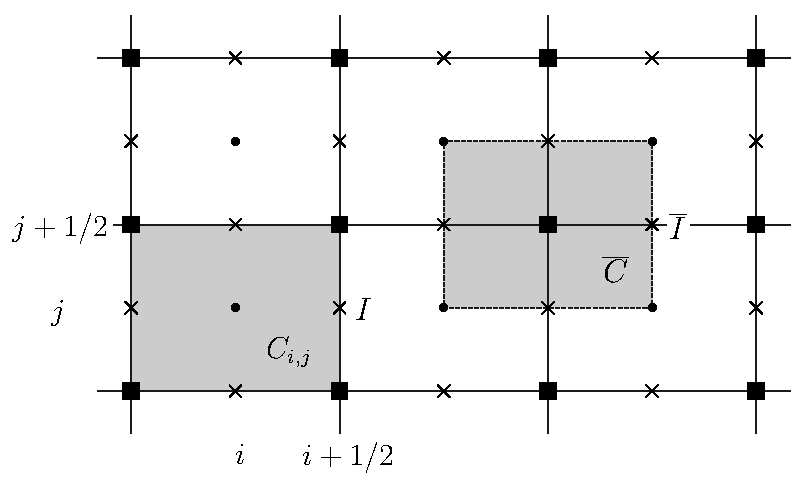
\includegraphics{Graphics/Grid}
\caption{Cartesian grid arrangement for two space dimensions. 
$C_{i,j}$: primary finite volumes, 
$\ \bullet\ $: primary cell centers, $I$: primary cell interfaces,
$\times$: centers of both primary and dual cell interfaces, 
$\overline{C}$: dual cells for nodal pressure computation, $\ \rule[1pt]{4pt}{4pt}\ $:
dual cell centers, $\overline{I}$: dual cell interfaces.
\label{fig:GridArrangement}}
\end{figure}

The space discretization of the present scheme is fully cell-centered 
on control volumes $C_{i,j,k}$ formed by a Cartesian mesh with constant 
grid spacings $\dx, \dy, \dz$, and grid indices $i = 0, ..., I-1$,  
$j = 0, ..., J-1$, $k = 0, ..., K-1$ in the three coordinate directions
(see Fig.~\ref{fig:GridArrangement} for a sketch of a two dimensional $x$-$y$ slice). 
The primary variables of the discrete approximate solution consists of grid cell 
averages 
%
\begin{equation}
\Sol_{i,j,k}^n \approx 
\frac{1}{\dx \dy \dz}\int\limits_{C_{i,j,k}} \Sol(\vx,t^n)\, d^3\vx
\qquad\text{of}\qquad 
\Sol = \left(
\begin{array}{c}
\rho \\ \rho\vu \\ \rho w \\ P \\ P\chiprime
\end{array}
\right)\,.
\end{equation}
%
The scheme is second-order accurate, so that -- within the approximation
order -- we can interchangeably interpret $\Sol_{i,j,k}^n$ as the cell average
or as a point value of $\Sol$ at the center of mass of the grid 
cell.  

Advection of the specific variables $\Psi$ defined in \eq{eq:PsiDefinition} is mediated by fluxes defined 
on cell faces, i.e.,
%
\begin{equation}\label{eq:DiscreteAdvectiveFluxes}
(Pu \Psi)^{n+\half}_{i+\half,j,k}\,,
\qquad
(Pv \Psi)^{n+\half}_{i,j+\half,k}\,, 
\qquad
(Pw \Psi)^{n+\half}_{i,j,k+\half}\,,
\end{equation}
%
determined by any second-order advection scheme. See 
section~\ref{sssec:AdvectiveFluxes} for the present implentation using
a ``monotone upwind scheme for conservation laws'' (MUSCL) 
following, e.g., \citet{vanLeer2006}. 
The fluxes in \eq{eq:DiscreteAdvectiveFluxes} are staggered-grid 
components of the advective flux field $(P\vv)^{n+\half}$ referred
to in section~\ref{sec:TimeDiscretizationSummary}\ref{ssec:TimeDiscretizationOverview} above. See
Fig.~\ref{fig:GridArrangement} for their arrangement on the computational 
grid.

Two different incarnations of the Exner pressure gradient are needed in 
the implicit Euler steps summarized in \eq{eq:HalfTimePredictorFluxCorrection} 
and \eq{eq:ImplicitEulerStep}. The former determines the cell interface
based fluxes from \eq{eq:DiscreteAdvectiveFluxes} and naturally works with 
cell- and timestep-centered values of the Exner pressure $\left(\pi_{i,j,k}^n\right)$. 
The latter corrects the cell-centered momenta and requires integrals of the Exner 
pressure over grid cell faces to form a finite-volume discretization of 
the gradient, and this is computed from node-centered values by the 
trapezoidal rule quadrature. Thus we compute both
%
\begin{equation}\label{eq:ExnerPressures}
\pi_{i,j,k}^{n+\half} 
\qquad\text{and}\qquad
\pi_{i+\half,j+\half,k+\half}^{n+1} 
\end{equation}
%
in the course of a time step $t^{n} \to t^{n+1}$ by solving implicit 
pressure equations. 

% ===========================================================================
% ===========================================================================

\subsection{Synchronization of auxiliary variables}
\label{ssec:Synchronization}

The fluid dynamical pressure $p$  plays multiple roles in the compressible 
Euler equations as formulated in \eq{eq:CompressibleEuler}. The cell-centered 
volume average of $P = (\rfr{p}/R) (p/\rfr{p})^{c_v/c_p}$ is representative 
of the internal energy budget of the flow \benacchio{(can we not frame the first part
of the sentence in terms of Exner already?)}, whereas the gradient of the Exner 
pressure $\pi = (p/\rfr{p})^{R/c_p}$ arises in the coupling of the momentum 
field to the pressure. As a consequence, the implicit Euler steps control both 
the advective fluxes $(P\vv)^{n+\half}$ at cell faces in 
\eq{eq:HalfTimePredictorFluxCorrection} and the momenta $(\rho \vv)$ at the 
cell centers in \eq{eq:TimeIntegrator}, thereby employing both cell-centered
and node-centered approximations of the Exner pressure, see \eq{eq:ExnerPressures} 
and sections~\ref{sssec:DivControlledAdvectiveFluxes} and 
\ref{sssec:TrapezoidalRule} below. This is in agreement with our previous
developments in \cite{KleinTCFD2009,BenacchioEtAl2014}, and with the 
established combination of ``MAC'' and cell-centered projections for 
zero Mach number flow solvers in \citep[e.g.,][]{BellEtAl1989,AlmgrenEtAl2006}.

These auxiliary fields are synchronized upon completion of the $n$th time
step with the primary cell centered variable $P^n_{i,j}$ through
%
\begin{IEEEeqnarray}{rCl}
\pi^{n}_{i,j,k} 
  & =
    & \left(\frac{RP_{i,j,k}^n}{\rfr{p}}\right)^{\frac{R}{c_v}}
      \IEEEyesnumber\IEEEyessubnumber*\\[10pt]
\pi^{n}_{i+\half,j+\half,k+\half}
  & =
    & \frac{1}{8}
      \sum_{\lambda,\mu,\nu = 0}^1 \pi^{n}_{i+\lambda,j+\mu,k+\nu} \,. 
%      \left(\pi^{n}_{i,j} + \pi^{n}_{i+1,j} + \pi^{n}_{i,j+1} + \pi^{n}_{i+1,j+1} 
%      \right)\,.
      \label{eq:CenterToNodeInterpolation}
\end{IEEEeqnarray}
%
The formula in \eq{eq:CenterToNodeInterpolation} is also used to generate 
half time level nodal pressures from the cell-centered solution 
$\pi^{n+\half}_{i,j,k}$ arising in the advective flux 
calculation scheme in \eq{eq:HalfTimePredictorFluxCorrection}, 
\eq{eq:HalfTimePredictorPLinearization}.

\benacchio{\eq{eq:CenterToNodeInterpolation} to be removed if effectively not used.}

Similarly, the split of the full inverse of the potential temperature 
$\chi = \chiprime + \chibar$ according to \eq{eq:PerturbationVariables} and the subsequent 
separate updates of  $\chi$ and $\chiprime$ governed by discrete versions
of the full and perturbed mass balances in \eq{eq:chiI} and 
\eq{eq:EulerPChiPrime}, respectively, require re-synchronization. Thus, 
after completion of a time step we let
%
\begin{equation}
\chiprime_{i,j,k}^{n} = \chi_{i,j,k}^{n} - \chibar_{k}^{n}\,,
\end{equation}   
%
where we have assumed gravity to be aligned with the $z$-coordinate
direction so that the discrete version of $\chibar(z)$ depends on the 
associated index $k$ only. Also, in 
all subsequent simulations we set $\chibar_k^{n} \equiv \chibar_k^{0}$.
An alternative option better suited for large scale, long time simulations 
is to invoke a horizontal, possibly local, averaging procedure to extract 
$\chibar$ from $\chi$ at least every few time steps. We leave testing 
this option to future work.	 

% ===========================================================================
% ===========================================================================

\subsection{Advection}
\label{ssec:Advection}

Any robust numerical scheme capable of performing advection of a scalar in
compressible flows is a good candidate for the generic discrete
advection operators $\mathcal{A}_{\text{1st}}^{\dt}$ and 
$\mathcal{A}_{\text{2nd}}^{\dt}$ introduced above. EULAG uses 
variants of the ``multi-dimensional positive definite advection transport 
algorithm'' (MPDATA, \citet{PrusaEtAl2008}). The present implementation involves
a directionally split ``monotone upwind scheme for conservation laws'' (MUSCL, see, e.g.,
\citet{vanLeer2006}): 

Suppose the half-time predictor step from \eq{eq:HalfTimePredictorFluxCorrection}, 
the details of which will be described shortly, has been completed. Then, 
the components of the advecting fluxes $(P\vv)^{n+\half}$ at grid cell faces 
have become available as part of this calculation. Given these fluxes, the advection 
step in \eq{eq:AdvectionStep} is discretized via Strang splitting, so that
%
\begin{equation}\label{eq:AdvectionStrangSplitting}
\Sol_{i,j}^{**} 
=
\mathcal{A}_{2\text{nd}}^{\dt} \Sol_{i,j,k}^{*} 
\equiv
\mathcal{A}^{\frac{\dt}{2}}_x 
\mathcal{A}^{\frac{\dt}{2}}_y 
\mathcal{A}^{\frac{\dt}{2}}_z 
\mathcal{A}^{\frac{\dt}{2}}_z 
\mathcal{A}^{\frac{\dt}{2}}_y 
\mathcal{A}^{\frac{\dt}{2}}_x\, \Sol_{i,j}^{*} \,,
\end{equation}
%
where, dropping the indices of the transverse directions 
for simplicity, we have, e.g., 
%
\begin{equation}
\mathcal{A}^{\frac{\dt}{2}}_x\, \Sol_{i} 
= \Sol_{i}
- \frac{\dt}{2\dx} 
  \left((Pu)^{n+\half}_{i+\half}\, \Psi_{i+\half} 
      - (Pu)^{n+\half}_{i-\half}\, \Psi_{i-\half} \right)
\end{equation}
%
with 
%
\begin{IEEEeqnarray}{rCl}\label{eq:AdvSpecifics}
\Psi_{i+\half} 
  & = 
    & \sigma \Psi^{-}_{i+\half} + (1-\sigma)\Psi^{+}_{i+\half}\,,
      \IEEEyesnumber\IEEEyessubnumber*\\[8pt]
\sigma 
  & = 
    & \text{sign}\left((Pu)^{n+\half}_{i+\half}\right)\,,
      \\[8pt]
\Psi^{-}_{i+\half} 
  & = 
    & \Psi_{i} + \frac{\dx}{2} \left(1 - C^{n+\half}_{i+\half} \right)  s_{i}\,,
      \\[8pt]
\Psi^{+}_{i+\half} 
  & = 
    & \Psi_{i+1} - \frac{\dx}{2} \left(1 + C^{n+\half}_{i+\half} \right)  s_{i+1}\,,
      \\[8pt]
C^{n+\half}_{i+\half}
  & =
    & \frac{\dt}{\dx} \frac{(Pu)^{n+\half}_{i+\half}}{(P_{i} + P_{i+1})/2}\,,
      \label{eq:AdvSpecificsCourantNo}\\[8pt]
s_{i}
  & =
    & \text{Lim}
      \left(\frac{\Psi_{i}-\Psi_{i-1}}{\dx}, \frac{\Psi_{i+1}-\Psi_{i}}{\dx}\right)\,,
      \label{eq:AdvSpecificsSlopes}
\end{IEEEeqnarray}
%
where $P_{i}$ in \eq{eq:AdvSpecificsCourantNo} denotes the fourth component 
of $\Sol_{i}$, and $\text{Lim}(a,b)$ is a slope limiting function 
\citep[see, e.g.,][]{Sweby1984}.

Importantly, the advecting fluxes $(P\vv)^{n+\half}$ are maintained unchanged 
throughout the Strang splitting cycle \eq{eq:AdvectionStrangSplitting}.

The first order accurate advection operator $\mathcal{A}_{1\text{st}}^{\dt}$
used in \eq{eq:HalfTimePredictorAdvection} is a simplified version
of the above in that (i) the advective fluxes are approximated at the old time level,
e.g.,
%
\begin{IEEEeqnarray}{rCl}\label{eq:firstorder_Adv}
(Pu)^{n}_{i+\half,j,k} 
  & = 
    & \frac{1}{2}\left((Pu)^{n}_{i,j,k} + (Pu)^{n}_{i+1,j,k}\right)\,,
\end{IEEEeqnarray}
%
and (ii) we use straightforward sequential instead of Strang splitting, i.e.,  
%
\begin{equation}
\mathcal{A}_{1\text{st}}^{\frac{\dt}{2}}
=
\mathcal{A}^{\frac{\dt}{2}}_x 
\mathcal{A}^{\frac{\dt}{2}}_y 
\qquad\text{and}\qquad
s_{i,j} \equiv 0\,,
\end{equation}
%
in our standard configuration. 
% ===========================================================================
% ===========================================================================

\subsection{Semi-implicit integration of the forcing terms}
\label{ssec:SemiImplicitForcing}

The generalized forcing terms on the right-hand side of \eq{eq:EulerP} are 
discretized in time by the implicit trapezoidal rule. This requires an explicit 
Euler step at the beginning and an implicit Euler step at the end of a time step. 
The implicit Euler step is also needed to compute the fluxes $(P\vv)^{n+\half}$ 
at the half time level as needed for the advection substep. In 
section~\ref{sssec:ImplicitEuler}) we summarize this implicit step in a 
temporal semi-discretization. Depending on whether this scheme is used to 
obtain stable advective fluxes or to complete the trapezoidal rule for the 
cell-centered momenta, the space discretization differs as outlined in 
sections~\ref{sssec:DivControlledAdvectiveFluxes}) and 
\ref{sssec:TrapezoidalRule}), respectively. 

% ===========================================================================

\subsubsection{Implicit Euler step in the temporal semi-discretization}
\label{sssec:ImplicitEuler}

Since both $\rho$ and $P$ are frozen in this split step because their 
evolution equations \eq{eq:EulerPMass} and \eq{eq:EulerPP} do not carry a 
right hand side, the relevant linearized equations, including the 
auxiliary potential temperature perturbation equation \eq{eq:EulerPChiPrime} 
may be written as 
%
\begin{IEEEeqnarray}{rCl}\label{eq:LinearizedNonAdvectiveSystem}
U_t
  & = 
    & - c_p (P\Theta)^* \pi'_x + f V
      \IEEEyesnumber\IEEEyessubnumber*\\[7pt]
V_t
  & = 
    & - c_p (P\Theta)^* \pi'_y - f U
      \\[0pt]
W_t
  & =
    & - c_p (P\Theta)^* \pi'_z + g \frac{\Thetatilde}{\Thetabar}
      \\
\Thetatilde_t
  & =
    & - W\frac{d\Thetabar}{dz}
      \\
\left(\frac{\partial P}{\partial \pi}\right)^*\pi'_t
  & =
    & - U_x - V_y - W_z\,,
\end{IEEEeqnarray}
%
where we have abbreviated
%
\begin{equation}
(U,V,W,\Thetatilde) = (P u, P v, P w, P(1/\chi)')\,,
\end{equation}
%
and where the coefficients $(P\Theta)^*$ and $(\partial P/\partial \pi)^*$ 
are prescribed or can be adjusted nonlinearly in an outer iteration loop 
as described in a similar context by \citet{SmolarkiewiczEtAl2014} \benacchio{Are these starred variables the same as in \eqref{eq:ExplicitEulerStep} or a general base state?}.
\klein{\bfseries This is a good question, and there is some ambiguity: In the first
projection (see file flux\_correction.c, and in there routine operator\_coefficients(), 
I am using $P$ from the old time level, and $Y$ -- that is $\chi$ -- from the current
field. In the second projection, I am using values from the current field throughout. 
For the second projection, this is what we should do, because $P$ and $\rho$ have their
final $t^{n+1}$ values after the advection sweep, and we are only updating the cell-centered
momenta and the nodal pressure. In the first projection, one can play with how to choose 
the starred coefficients. In practice, I have seen hardly a difference so far. But this 
may have changed in the meantime. I have not tested this in quite some time and the scheme
has developed substantially in other parts of the code. Actually, in operator\_coefficients()
you will find compiler directives by which you can already switch to a different option for
evaluating these coefficients.}
 The 
implicit Euler semi-discretization of \eq{eq:LinearizedNonAdvectiveSystem} 
in time reads
%
\begin{IEEEeqnarray}{rCl}\label{eq:LinearizedNonAdvectiveImplicitEuler}
U^{n+1}
  & = 
    & U^{n} - \dt \left( c_p (P\Theta)^* {\pi'}^{n+1}_x - f V^{n+1}\right)
      \IEEEyesnumber\IEEEyessubnumber*\\[7pt]
V^{n+1}
  & = 
    & V^n - \dt \left( c_p (P\Theta)^* {\pi'}^{n+1}_y + f U^{n+1} \right)
      \\[0pt]
W^{n+1}
  & =
    &  W^n - \dt 
       \left( c_p (P\Theta)^* {\pi'}^{n+1}_z - g \frac{{\Thetatilde}^{n+1}}{\Thetabar} 
       \right)
      \\
{\Thetatilde}^{n+1}
  & =
    & {\Thetatilde}^{n} - \dt\frac{d\Thetabar}{dz}\, W^{n+1}
      \\
\left(\frac{\partial P}{\partial \pi}\right)^* {\pi'}^{n+1}
  & =
    & \left(\frac{\partial P}{\partial \pi}\right)^* {\pi'}^{n} 
    - \dt \left( U^{n+1}_x + V^{n+1}_y + W^{n+1}_z \right)\,.
    \label{eq:LinearizedNonAdvectiveImplicitEulerPi}
\end{IEEEeqnarray}
%
Straightforward manipulations yield the new time 
level velocity components, 
%
\begin{IEEEeqnarray}{rCl}\label{eq:LinearizedNonAdvectiveImplicitEulerSolI}
\left(
\begin{array}{c}
U \\ V
\end{array}
\right)^{n+1} 
  & =
    &  \frac{1}{1+(\dt f)^2}
      \left[
      \left(
        \begin{array}{c}
        U + \dt\, f\, V \\ 
        V - \dt\, f\, U
        \end{array}
      \right)^n
    - \dt \, c_p (P\Theta)^* 
      \left(
        \begin{array}{c}
        \pi'_x + \dt\, f\, \pi'_y \\ 
        \pi'_y - \dt\, f\, \pi'_x
        \end{array}
      \right)^{n+1}
      \right] \quad
      \IEEEyesnumber\IEEEyessubnumber*\\
W^{n+1} 
  & =
    & \left(\frac{W + \dt\, g {\Thetatilde}/\Thetabar}{1 + (\dt\, N)^2}\right)^n
      - \dt \, \frac{c_p (P\Theta)^*}{1 + (\dt\, N)^2} \ {\pi'}^{n+1}_z \,. 
\end{IEEEeqnarray}
%
Insertion of the expressions in \eq{eq:LinearizedNonAdvectiveImplicitEulerSolI}
into the pressure equation \eq{eq:LinearizedNonAdvectiveImplicitEulerPi} 
leads to a closed Helmholtz-type equation for ${\pi'}^{n+1}$. After its 
solution, backward re-insertion yields $(U, V, W, \Thetatilde)^{n+1}$. 
Specifically, 
%
 \begin{multline}\label{eq:helmholtz}
 \left(\dfrac{\partial P}{\partial\pi}\right)^*\pi'^{n+1} - \\
\left\{
    \dfrac{c_p\dt^2}{1+(\dt f)^2} 
    \left\{
      \left[
        \left(P\Theta\right)^*
          \left(\pi'^{n+1}_x+\dt f\pi'^{n+1}_y
          \right)
        \rule{0pt}{12pt}\right]_x
       +\left[
          \left(P\Theta\right)^*
            \left(\pi'^{n+1}_y-\dt f\pi'^{n+1}_x
            \right)
         \rule{0pt}{12pt}\right]_y
      \right\}
    \right.\\
    \left.
  + \dfrac{c_p\dt^2}{1+(\dt N)^2}
      \left[\left(P\Theta\right)^*\pi'^{n+1}_z
      \rule{0pt}{12pt}\right]_z
    \right\}
  = R^n
 \end{multline}
%
with the right-hand side:
%
\begin{multline}\label{eq:helmholtz_rhs}
R^n=\left(\dfrac{\partial P}{\partial\pi}\right)^*\pi'^n-\\
\left\{\dfrac{\dt}{1+(\dt f)^2}\left[U^n_x+V^n_y+\dt f(V^n_x-U^n_y)\right]
+\dfrac{\dt}{1+(\dt N)^2}\left[W^n_z+\dt\, g\left(\Thetatilde/\Thetabar\right)^n_z\right]\right\} \,.
\end{multline}
%% ===========================================================================

\subsubsection{Divergence controlled advective fluxes via 
\eq{eq:HalfTimePredictorFluxCorrection}}
\label{sssec:DivControlledAdvectiveFluxes}

Advection is discretized using standard cell-centered flux divergences.  
Thus, the divergence of, e.g., the vector field $\vV = (U,V,W)$ uses the 
discrete approximation
%
\begin{equation}
\widetilde{\left(U_x\right)}_{i,j,k} 
=
\frac{1}{\dx} \left(U_{i+\half,j,k} - U_{i-\half,j,k}\right)\,,
\end{equation}
%
and analogous expressions for $V_y$ and $W_z$.

Correspondingly, \eq{eq:HalfTimePredictorFluxCorrection} determines the 
half time level advecting flux components located at the grid cell faces 
using a first order accurate time integrator to lift the data from time 
level $t^n$ to $t^{n+\half}$. Having completed the advection predictor, 
\eq{eq:HalfTimePredictorAdvection}, we first generate face centered 
approximations of the advective fluxes,
%
\begin{IEEEeqnarray}{rClCrCl}\label{eq:InterpolationToCellFaces}
(Pu)^{\#}_{i+\half,j,k} 
  & = 
    & \frac{1}{2} 
      \left[(\rho u\chi)^{\#}_{i,j,k} + (\rho u\chi)^{\#}_{i+1,j,k}
      \right]\,, 
\end{IEEEeqnarray}
%
and analogous expressions for the other Cartesian directions.
These differ from the corresponding data at time
level $t^n$ through the effect of the advection step only, so that a consistent
first order approximation at $t^{n+\half}$ requires us to account for the
influence of the right hand side $Q$ of the advection equation with forcing in 
\eq{eq:EulerPCompactPsi} as well. 
This is achieved through a linearized implicit Euler step as described in 
point~\ref{sssec:ImplicitEuler}) above. 

The components $(U,V,W)$ of $(P\vv)$ in this calculation are located at
the cell faces, so that an appropriate spatial discretization of the
pressure gradient is obtained from cell-centered values as
%
\begin{equation}
\widetilde{\left(\pi'_x\right)}_{i+\half,j,k} 
= 
\frac{1}{\dx} \left(\pi'_{i+1,j,k} - \pi'_{i,j,k}\right)\,,
\end{equation}
%
with analogous expressions for the other Cartesian directions, 
and this leads to standard five-point (respectively seven-point) discrete Laplacians in 
two (respectively three) space dimensions. We have also implemented the
alternative approximation
%
\begin{equation}\label{eq:NinePointStencilI}
\widetilde{\left(\pi'_x\right)}_{i+\half,j,k} 
\approx 
\frac{1}{\dx} \left({\pibar}^{x,\prime}_{i+1,j,k} - {\pibar}^{x,\prime}_{i,j,k}\right)\,,
\end{equation}
%
where
%
\begin{IEEEeqnarray}{rCl}\label{eq:NinePointStencilII}
{\pibar}^{x,\prime}_{i,j,k} = \frac{36}{64} \pi'_{i,j,k} 
  & + 
    & \frac{6}{64} \left(\pi'_{i,j+1,k} + \pi'_{i,j-1,k} + \pi'_{i,j,k+1} + \pi'_{i,j,k-1}\right)
      \\
  & +
    & \frac{1}{64} 
      \left(\pi'_{i,j+1,k+1} + \pi'_{i,j-1,k+1} + \pi'_{i,j+1,k-1} + \pi'_{i,j-1,k-1}
      \right)\,,
    \IEEEnonumber
\end{IEEEeqnarray}
%
and analogous formulae for the other Cartesian directions.
This leads to nine- and twentyseven-point discrete Laplacians in 
two and three dimensions, respectively, and corresponds to finite
volume approximations of the gradient based on bi- and trilinear 
approximations of the pressure field between cell centers. 
See \citep{Sueli1991} for related numerical analysis and
\citep{VaterKlein2009,KleinTCFD2009,BenacchioEtAl2014} for our
earlier experiences with this approach. Results presented in this paper
are based on \eq{eq:NinePointStencilI}, \eq{eq:NinePointStencilII}.

The coefficients $(P\Theta)^*$ and the explicit contributions with
superscript $\left(\cdot\right)^n$ in 
\eq{eq:LinearizedNonAdvectiveImplicitEulerSolI} are evaluated first
at the cell centers and then interpolated to the cell faces in
analogy with \eq{eq:InterpolationToCellFaces}. In contrast, the 
linearization term from the equation of state, 
$\left(\partial P/\partial \pi\right)^*$ is needed and evaluated 
directly at the cell centers.

% ===========================================================================

\subsubsection{Pressure gradient and divergence computation in the generalized sources}
\label{sssec:TrapezoidalRule}

The linearized equations for inclusion of the source terms in
\eq{eq:LinearizedNonAdvectiveSystem} need to be evaluated at the
cell centers when we apply the two steps of the trapezoidal rule 
in \eq{eq:ExplicitEulerStep} and \eq{eq:ImplicitEulerStep}. To 
this end, the coefficients $(P\Theta)^*$ are evaluated at the 
cell centers as well, the linearization term from the equation of state
$\left(\partial P/\partial \pi\right)^*$ is interpolated from 
the cell centers to the nodes in analogy with the pressure 
interpolation \eq{eq:CenterToNodeInterpolation}, and the components
of the pressure gradient are approximated as
%
\begin{IEEEeqnarray}{rCl}
\left(\pi'_x\right)_{i,j,k} 
  & = 
    & \frac{1}{\dx} \left(\piprimehat_{i+\halff,j,k} - \piprimehat_{i-\halff,j,k}\right)
      \IEEEyesnumber\IEEEyessubnumber*\\
\piprimehat_{i+\halff,j,k} 
  & = 
    & \frac{1}{4}
      \left(\pi'_{i+\halff,j+\halff,k+\halff} + \pi'_{i+\halff,j-\halff,k+\halff}
          + \pi'_{i+\halff,j+\halff,k-\halff} + \pi'_{i+\halff,j-\halff,k-\halff}
      \right)\,.
\end{IEEEeqnarray}
%
Analogous formulae hold for the other Cartesian directions. The divergence
in \eq{eq:LinearizedNonAdvectiveImplicitEulerPi} is formed on the basis 
of the cell-centered components of $\vV = (U,V,W)$, with 
%
\begin{IEEEeqnarray}{rCl}
\left(U_x\right)_{i+\halff,j+\halff,k+\halff} 
  & = 
    & \frac{1}{\dx} \left(\Uhat_{i+1,j+\halff,k+\halff} - \Uhat_{i,j+\halff,k+\halff}\right)
      \IEEEyesnumber\IEEEyessubnumber*\\
\Uhat_{i,j+\halff,k+\halff} 
  & = 
    & \frac{1}{4}
      \left(U_{i,j+1,k+1} + U_{i,j-1,k+1} + U_{i,j+1,k-1} + U_{i,j-1,k-1}
      \right)\,.
\end{IEEEeqnarray}
%
and analogous formulae for the other Cartesian directions.
This leads to a node-centered discretization of the pressure Helmholtz 
equation based on a nine- (respectively 27)-point stencil of the Laplacian.
The solution gives the required update of the node-centered perturbation 
pressure field. 

\subsection{Tabular summary of the numerical scheme}

In the following we summarize the operations in one time step of the algorithm described above%

\vspace{2 mm}

\newpage

\begin{falgorithm}[Compressible scheme]
\ \\
% Starting from compliant initial and boundary conditions:
\begin{description}
%
\vspace{-2mm}

\item[\emph{Initialization}]\ \\ Grid setting and input preprocessing. Optional first elliptic solve to generate a divergence-improved velocity field. Then, for each time loop, \textbf{do}:
%
\item[\emph{First stage}]
%
  \begin{enumerate}\item[]
    \item[(i)] Determine advective fluxes $(P\vv)^{n+1/2}$ in \eq{eq:HalfTimePredictorFluxCorrection} using scalars computed in \eq{eq:HalfTimePredictorAdvection}.  

    \item[(ii)] Use the relation between $P$ and $\pi$ in \eq{eq:HalfTimePredictorPLinearization} to construct a first Helmholtz problem for the half-time level pressure $\pi^{n+1/2}$.

    \item[(iii)] Use the advective fluxes to obtain $P^{n+1}$ through \eq{eq:PUpdate}.

  \end{enumerate}

\item[\emph{Second stage - scalars update}]
%
  \begin{enumerate}\item[]
    \item[(i)] Evolve the scalars $\Psi$ as defined in \eq{eq:PsiDefinition} to the new time-level using the explicit-then-advection-then-implicit procedure of \eq{eq:ExplicitEulerStep}-\eq{eq:AdvectionStep}-\eq{eq:ImplicitEulerStep}

    \item[(ii)] In \eq{eq:ImplicitEulerStep} for the momentum-like components of $\Psi$, a second Helmholtz problem \eq{eq:helmholtz} is constructed to find $\pi'^{n+1}$.

  \end{enumerate}

\item[\emph{Auxiliary variables update}]

  \begin{enumerate}\item[]
    \item[(i)] The auxiliary variables $(\chi', \piprime)$ are computed from the primary unknowns at the new time level.
  \end{enumerate}

%
%\item[\emph{Conclusion}]\ \\ Post-processing and output management.  
%
\end{description}
\end{falgorithm}


%% If more than one appendix, use \appendix[<letter>], e.g.,
% \appendix[A] 

%\appendixtitle{Title of Appendix}


%\subsection{Appendix section}

%%%%%%%%%%%%%%%%%%%%%%%%%%%%%%%%%%%
%APPENDIX FIGURE AND TABLE EXAMPLES---PLACE AT END OF DOCUMENT
%%%%%%%%%%%%%%%%%%%%%%%%%%%%%%%%%%%
%
%\begin{table}
%\appendcaption{A1}{Here is the appendix table caption.}
%\centering
%\begin{tabular}{ccc}
%a&b&c\\
%d&e&f
%\end{tabular}
%\end{table}
%
%\begin{figure}
%\centerline{(illustration here)}
%\appendcaption{A1}{Here is the appendix figure caption.}
%\end{figure}



\end{document}
%%%%%%%%%%%%%%%%%%%%%%%%%%%%%%%%%%%%%%%%%%%%%%%%%%%%%%%%%%%%%%%%%%%%%
% END OF HYDRO_COMP_NUMERICS_MWR.TEX
%%%%%%%%%%%%%%%%%%%%%%%%%%%%%%%%%%%%%%%%%%%%%%%%%%%%%%%%%%%%%%%%%%%%%